\documentclass[12pt]{article}
\usepackage[utf8]{inputenc}

\usepackage{lmodern}

\usepackage{enumitem}
\usepackage[margin=2cm]{geometry}

\usepackage{amsmath, amsfonts, amssymb}
\usepackage{graphicx}
%\usepackage{subfigure}
\usepackage{tikz}
\usepackage{pgfplots}
\usepackage{multicol}

\usepackage{comment}
\usepackage{url}
\usepackage{calc}
\usepackage{subcaption}
\usepackage[indent=0pt]{parskip}
\usepackage{animate}

\usepackage{array}
\usepackage{blkarray,booktabs, bigstrut}
\usepackage{bigints}

\pgfplotsset{compat=1.16}

% MATH commands
\newcommand{\ga}{\left\langle}
\newcommand{\da}{\right\rangle}
\newcommand{\oa}{\left\lbrace}
\newcommand{\fa}{\right\rbrace}
\newcommand{\oc}{\left[}
\newcommand{\fc}{\right]}
\newcommand{\op}{\left(}
\newcommand{\fp}{\right)}

\newcommand{\bi}{\mathbf{i}}
\newcommand{\bj}{\mathbf{j}}
\newcommand{\bk}{\mathbf{k}}
\newcommand{\bF}{\mathbf{F}}

\newcommand{\mR}{\mathbb{R}}

\newcommand{\ra}{\rightarrow}
\newcommand{\Ra}{\Rightarrow}

\newcommand{\sech}{\mathrm{sech}\,}
\newcommand{\csch}{\mathrm{csch}\,}
\newcommand{\curl}{\mathrm{curl}\,}
\newcommand{\dive}{\mathrm{div}\,}

\newcommand{\ve}{\varepsilon}
\newcommand{\spc}{\vspace*{0.5cm}}

\DeclareMathOperator{\Ran}{Ran}
\DeclareMathOperator{\Dom}{Dom}

\newcommand{\exo}[1]{\noindent\textcolor{red}{\fbox{\textbf{Problem {#1}}}\hrulefill}\\}
\newcommand{\qu}[4]{\noindent\textcolor{#4}{\fbox{\textbf{Section {#1} | Problem {#2}}} \hrulefill{{\fbox{\textbf{{#3} Points}}}}\\}}

\newcommand{\semester}{Spring 2023}

\newcommand{\CVup}{%

\begin{tikzpicture}
\draw[black, <->, >=latex] (-0.33, 0.5) .. controls (-0.125, 0) and (0.125, 0) .. (0.33, 0.5);
\end{tikzpicture}}

\newcommand{\CVupInc}{%
\begin{tikzpicture}
\draw[black, ->, >=latex] (0,0) .. controls (0.2, 0) and (0.4, 0.2) .. (0.5, 0.5);
\end{tikzpicture}}

\newcommand{\CVupDec}{%
\begin{tikzpicture}[rotate=270]
\draw[black, ->, >=latex] (0,0) .. controls (0.2, 0) and (0.4, 0.2) .. (0.5, 0.5);
\end{tikzpicture}}

\newcommand{\CVdown}{%
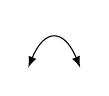
\begin{tikzpicture}
\draw[black, <->, >=latex] (-0.33, -0.5) .. controls (-0.125, 0) and (0.125, 0) .. (0.33, -0.5);
\end{tikzpicture}}

\newcommand{\CVdownInc}{%
\begin{tikzpicture}
\draw[black, ->, >=latex] (-0.5, -0.5) .. controls (-0.5, -0.3) and (-0.5, -0.1) .. (0,0);
\end{tikzpicture}}

\newcommand{\CVdownDec}{%
\begin{tikzpicture}[rotate=-90]
\draw[black, ->, >=latex] (-0.5, -0.5) .. controls (-0.5, -0.3) and (-0.5, -0.1) .. (0,0);
\end{tikzpicture}}

\begin{document}
	\noindent \hrulefill \\
	MATH-241 \hfill Pierre-Olivier Paris{\'e}\\
	Solutions Section 3-3 \hfill \semester \\\vspace*{-1cm}
	
	\noindent\hrulefill
	
	\spc
		
	\exo{10}
	\begin{enumerate}[label=\alph*)]
	\item The derivative of $f$ is 
		\begin{align*}
		f'(x) = 6x^2 - 18x + 12 .
		\end{align*}
	We see that 	
		\begin{align*}
		f'(x) = 6 (x - 3x + 2) = 6(x - 2) (x - 1) .
		\end{align*}
	Therefore, the zeros of $f'$ are $x = 2$ and $x = 1$. 
		\begin{itemize}
		\item if $x < 1$, then $x < 2$ also. Therefore, $x - 1 < 0$ and $x - 2 < 0$. The product $(x - 2) (x - 1)$ is positive, being the product of two negative quantities. So $f' (x ) > 0$ when $x < 1$. Hence $f$ is increasing for $x < 1$.
		\item if $x > 1$ and $x < 2$. Therefore, $x - 1 > 0$ and $x - 2 < 0$. The product $(x - 2) (x - 1)$ is negative, being the product of a negative quantity by a positive quantity. So $f'(x) < 0$ when $x > 1$ and $x < 2$. Hence $f$ is decreasing for $1 < x < 2$. 
		\item If $x > 2$, then $x > 1$ also. Therefore $x - 1 > 0$ and $x - 2 > 0$. The product $(x - 2) (x - 1)$ is positive, being the product of two positive quantities. So $f'(x) > 0$ when $x > 2$. Hence $f$ is increasing for $x > 2$. 
		\end{itemize}
	\item We know that $f'(x) = 6(x - 2) (x - 1)$. Therefore, the zeros of the derivative are $x = 1$ and $x = 2$. The derivative exists everywhere. 
		\begin{itemize}
		\item $x = 1$. In this case, we see that $f$ is increasing for $x < 1$ and $f$ is decreasing for $1 < x < 2$. Therefore, from the first derivative test, $f$ attains a local maximum at $x = 1$.
		\item $x = 2$. In this case, we see that $f$ is decreasing for $1 < x < 2$ and increasing for $x > 2$. Therefore, from the first derivative test, $f$ attains a local minimum at $x = 2$. 
		\end{itemize}
	\item The second derivative of $f$ is
		\begin{align*}
		f''(x) = 12x - 18 = 6 (2x - 3) .
		\end{align*}
	The zeros of $f''$ are $x = 3/2$.
		\begin{itemize}
		\item When $x < 3/2$, then $2x - 3 < 0$. Therefore, $f''(x) < 0$. This means that $f$ is concave downward.
		\item When $x > 3/2$, then $2x - 3 > 0$. Therefore, $f''(x) > 0$. This means that $f$ is concave up..
		\end{itemize}
	\end{enumerate}
	
	\newpage
	
	\exo{12}
	\begin{enumerate}[label=(\alph*)]
	\item The derivative of $f$ is
		\begin{align*}
		f'(x) = \frac{x^2 + 1 - 2x^2}{(x^2 + 1)^2} = \frac{1 - x^2}{(1 + x^2)^2} = \frac{(1 - x)(1 + x)}{(1 + x^2)^2} .
		\end{align*}
	The critical points are at $x = 1$ and $x = -1$ where $f'(x)$ is zero. The derivative exists for any $x$. 
	
	When $x < -1$, then $(1 - x) > 0$ and $1 + x < 0$. The denominator is always positive and therefore $f'(x) < 0$. The function is decreasing when $x < -1$.
	
	When $-1 < x < 1$, then $1 - x > 0$ and $1 + x > 0$. The denominator is always positive and therefore $f'(x) > 0$. The function is increasing for $-1 < x < 1$.
	
	When $x > 1$, then $1 - x < 0$ and $1 + x > 0$. The denominator is always positive and therefore $f'(x) < 0$. The function is decreasing for $x > 1$.
	
	\item When $x < -1$, the function $f$ is decreasing and when $-1 < x < 1$, the function $f$ is increasing. By the first derivative test, $x = -1$ is a local minimum. The local minimum value of $f$ there is therefore 
		\begin{align*}
		f(-1) = -\frac{1}{2} .
		\end{align*}
	
	When $-1 < x < 1$, the function $f$ is increasing and when $x > 1$, the function $f$ is decreasing. By the first derivative test, $x = 1$ is a local maximum. The local maximum value of $f$ there is
		\begin{align*}
		f (1) = \frac{1}{2} .
		\end{align*}
		
	\item The second derivative is
		\begin{align*}
		f''(x) &= \frac{-2x (1 + x^2)^2 - 4x (1 - x^2) (1 + x^2)}{(1 + x^2)^4} \\
		&= \frac{-2x (1 + 2x^2 + x^4) - 4x (1 - x^4)}{(1 + x^2)^4} \\
		&= \frac{-2x - 4x^3 - 4x^5 - 4x + 4x^5}{(1 + x^2)^4} \\
		&= \frac{-6x - 4x^3}{(1 + x^2)^4} \\
		&= -4\frac{x (3/2 - x^2)}{(1 + x^2)^4}
		\end{align*}
	and therefore 
		\begin{align*}
		f''(x) = -4 \frac{x (\sqrt{3/2} -  x) (\sqrt{3/2} + x)}{(1 + x^4)^4} .
		\end{align*}
	The possible inflection points are when $f''(x) = 0$ or $f''(x)$ does not exist. There is no problem with the expression of $f''(x)$. The zeros are $x = -\sqrt{3/2}$, $x =0$ and $x = \sqrt{3/2}$.
	
	Here is a table summarizing all the information we need to answer the question. The detailed explanations are presented after the table.
	\begin{center}
	\begin{tabular}{c||c|c|c|c|c|c|c}
	Factors & \phantom{22} $x < $ \phantom{22} & $-\sqrt{3/2}$ & \phantom{22} $< x < $ \phantom{22} & $0$ & \phantom{22} $< x < $ \phantom{22} & $\sqrt{3/2}$ & \phantom{22} $< x$ \phantom{22} \\\hline
	$-4$ & $-$ & $\cdot$ & $-$ & $\cdot$ & $-$ & $\cdot$ & $-$ \\
	$x$ & $-$ & $\cdot$ & $-$ & $\cdot$ & $+$ & $\cdot$ & $+$ \\
	$\sqrt{3/2} - x$ & $+$ & $\cdot$ & $+$ & $\cdot$ & $+$ & $\cdot$ & $-$ \\
	$\sqrt{3/2} + x$ & $-$& $\cdot$ & $+$ & $\cdot$ & $+$ & $\cdot$ & $+$ \\
	$(1 + x^4)^4$ & $+$ & $\cdot$ & $+$ & $\cdot$ & $+$ & $\cdot$ & $+$ \\\hline
	$f''(x)$ & $-$ & $0$ & $+$ & $0$ & $-$ & $0$ & $+$ \\
	$f(x)$ & \CVdown & IP & \CVup & IP & \CVdown & IP & \CVup
	\end{tabular}
	\end{center}
	
	When $x < -\sqrt{3/2}$, then $x < 0$, $\sqrt{3/2} - x > 0$, and $\sqrt{3/2} + x < 0$. Since $-4 < 0$ and the denominator is always positive, we conclude that $f''(x) < 0$. Therefore, the function is concave down for $x < -\sqrt{3/2}$.
	
	When $-\sqrt{3/2} < x < 0$, then $x < 0$, $\sqrt{3/2} - x > 0$ and $\sqrt{3/2} + x > 0$. Since $-4 < 0$ and the denominator is always positive, we conclude that $f''(x) > 0$ there. Therefore, the function is concave up for $-\sqrt{3/2} < x < 0$. 
	
	Since $f$ changes from concave down to concave up at $x = -\sqrt{3/2}$, the number $x = -\sqrt{3/2}$ is an inflection point.
	
	When $0 < x < \sqrt{3/2}$, then $x > 0$, $\sqrt{3/2} - x > 0$, and $\sqrt{3/2} + x > 0$. Since $-4 < 0$ and the denominator is always positive, we conclude that $f''(x) < 0$ there. Therefore, the function is concave  down for $0 < x < \sqrt{3/2}$.
	
	Since $f$ changes from concave up to concave down at $x = 0$, the number $x = 0$ is an inflection point.
	
	Finally, when $x > \sqrt{3/2}$, then $x > 0$, $\sqrt{3/2} - x < 0$, $\sqrt{3/2} + x > 0$. Since $-4 < 0$ and the denominator is always positive, we conclude that $f''(x) > 0$ there. Therefore, the function is concave up for $x > \sqrt{3/2}$.
	
	Since $f$ changes from concave down to concave up at $x = \sqrt{3/2}$, the number $x = \sqrt{3/2}$ is an inflection point.
	\end{enumerate}
	
	\spc
	
	\exo{16}
	\\
	\textbf{With the First Derivative Test.} The derivative of $f$ is
		\begin{align*}
		f'(x) = \frac{x(x - 2)}{(x - 1)^2} .
		\end{align*}
	The critical numbers of $f$ are $c = 0$, $c = 1$, and $ c= 2$.
	
		\begin{itemize}
		\item $c = 0$. 
			\begin{itemize}
			\item When $x < 0$, then $x - 2 < 0$. Since $(x - 1)$ is squared, then $(x - 1) > 0$. Therefore, we see that $f'(x) > 0$ for $x < 0$ because $f'(x)$ is the product of a two negative quantities and a positive quantity. So $f$ is increasing when $x < 0$.
			\item When $0 < x < 1$, then $x - 2 < 0$ and $x - 1 < 0$. But $(x - 1)$ is squared, so $(x- 1)^2 > 0$. Therefore, we see that $f'(x) < 0$ because $f'(x)$ is the product of two positive quantities and a negative quantity. Therefore, $f$ is decreasing if $0 < x < 1$. 
			\end{itemize}
		Using the First Derivative Test, we conclude that $c = 0$ is a local maximum of $f$.
	\item $c = 1$. 
		\begin{itemize}
		\item When $0 < x < 1$, then $x - 2 < 0$ and $x > 0$. Since $(x - 1)^2 > 0$, then $f'(x) < 0$ because it is a product of two positive quantities and a negative quantity. So $f$ is decreasing on $0 < x < 1$.
		\item When $1 < x < 2$, then $x - 2 < 0$ and $x > 0$. Since $(x - 1)^2 > 0$, then $f'(x) < 0$ because it is a product of two positive quantities and a negative quantity. So $f$ is decreasing on $1 < x < 2$. 
		\end{itemize}
		Since there is no change in the sign of $f'(x)$, we conclude that $c = 1$ is not a local maximum, nor a local minimum.
		\item $c = 2$. 
			\begin{itemize}
			\item When $1 < x < 2$, then $x - 2 < 0$ and $x > 0$. Since $(x - 1)^2 > 0$, then $f'(x) < 0$ because it is a product of two positive quantities and a negative quantity. So $f$ is decreasing on $1 < x < 2$. 
			\item When $x > 2$, then $x - 2 > 0$ and $x > 0$. Since $(x- 1)^2 > 0$, then $f'(x) > 0$ because it is the product of three positive quantities. So $f$ is increasing on $x > 2$.
			\end{itemize}
		By the First derivative Test, we conclude that $f$ has a local minimum at $c = 2$. 
		\end{itemize}
		
	\textbf{With the Second Derivative Test.} From the first part, we know that the critical numbers of $f$ are $c = 0$, $c = 1$, and $c = 2$. The second derivative of $f$ is
		\begin{align*}
		f''(x) = \frac{2}{(x - 1)^3} .
		\end{align*}
	\begin{itemize}
	\item $c = 0$. We have $f''(0) = \frac{2}{(-1)^3} = -2$. Since $f''(0) < 0$, by the Second Derivative Test, we conclude that $c = 0$ is a local maximum.
	\item $c = 1$. We have $f''(1)$ does not exist. So we can't conclude anything from the Second Derivative Test.
	\item $c = 2$. We have $f''(2) = \frac{2}{(1)^3} = 2$. Since $f''(2) > 0$, by the Second Derivative Test, we conclude that $c = 2$ is a local minimum.
	\end{itemize}
	
	\underline{Remark:} I personnaly prefer the Second Test Derivative over the First Derivative Test (but this is when we can use the second test).
		
	\newpage
	
	\exo{22}
	\\
	Here is a possible graph of a function with the desire properties.
	
	\begin{figure}[ht]
	\centering
	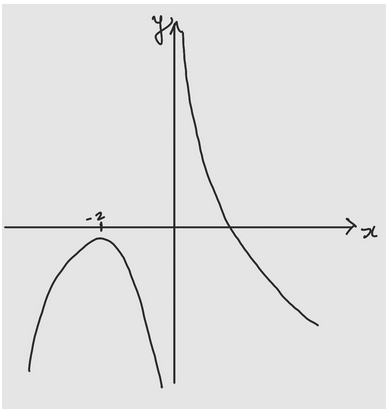
\includegraphics[scale=0.6]{number22.png}
	\end{figure}
	
	\spc
	
	\exo{30}
	\begin{enumerate}[label=(\alph*)]
	\item The derivative and the second derivative are positive at $B$. The reasons are that, at $B$, the slope of the tangent line is positive and the graph of the function is concave up.
	\item The derivative and the second derivative are negative at $E$. The reasons for that are, at $E$, the slope of the tangent line is negative and the graph of the function is concave down.
	\item The derivative is negative and the second derivative is positive at $A$. The reasons for that are, at $A$, the slope of the tangent line is negative and the graph of the function is concave up.
	\end{enumerate}
		
\end{document}